\documentclass[12pt,a4paper]{article}

\usepackage{fancyhdr}
\usepackage{graphicx}
\usepackage{placeins}
\usepackage{adjustbox}


\begin{document}

\pagestyle{fancy}
\fancyhf{}
\chead{Short summary report}

\begin{table}[t]
\centering
\caption {rnaQUAST metrics for assembled transcripts. In each row the best values are indicated with \textbf{bold}. For the transcript metrics (rows 4, 5, 6, 9, 13, 26, 27, 28) we highlighted the best \textbf{relative} values i.e. divided by the total number of transcripts in the corresponding assembly.}
\begin{adjustbox}{width=1\textwidth}
\small
\begin{tabular}{|l*{11}{|r}|}
\hline
\textbf{METRICS/TRANSCRIPTS}                            & \textbf{Trinity}       & \textbf{Trans-ABySS}   & \textbf{Oases}         & \textbf{SOAPdenovo-Trans} & \textbf{IDBA-Tran}     & \textbf{Bridger}       & \textbf{BinPacker}     & \textbf{Shannon}       & \textbf{rnaSPAdes}     & \textbf{SPAdes}        \\ \hline\hline
\multicolumn{11}{l}{\bf DATABASE METRICS}                                                 \\ \hline
Genes                                                   & 57992                  & 57992                  & 57992                  & 57992                  & 57992                  & 57992                  & 57992                  & 57992                  & 57992                  & 57992                  \\
Avg. number of exons per isoform                        & 5.971                  & 5.971                  & 5.971                  & 5.971                  & 5.971                  & 5.971                  & 5.971                  & 5.971                  & 5.971                  & 5.971                  \\ \hline
\multicolumn{11}{l}{\bf BASIC TRANSCRIPTS METRICS}                                        \\ \hline
Transcripts                                             & 365427                 & 1762439                & 1316143                & 1087869                & 281371                 & 277892                 & 27957                  & 162486                 & 668019                 & 353728                 \\
Transcripts $>$ 500 bp                                  & 113994                 & 151362                 & 479414                 & 65513                  & 71446                  & 92081                  & \textbf{26426}         & 54363                  & 112806                 & 82573                  \\
Transcripts $>$ 1000 bp                                 & 64061                  & 59779                  & 207474                 & 27529                  & 23516                  & 43201                  & \textbf{22611}         & 31328                  & 49860                  & 31039                  \\ \hline
\multicolumn{11}{l}{\bf ALIGNMENT METRICS}                                                \\ \hline
Aligned                                                 & 330366                 & 1606696                & 1209240                & 1008316                & 259491                 & 255022                 & \textbf{27709}         & 150324                 & 632083                 & 332617                 \\
Uniquely aligned                                        & 317880                 & 1576053                & 858267                 & 994920                 & 255855                 & 230696                 & 20274                  & 140216                 & 611585                 & 303526                 \\
Multiply aligned                                        & 2514                   & 18809                  & 10571                  & 8998                   & 2087                   & 1530                   & 43                     & 1451                   & 4264                   & 18281                  \\
Unaligned                                               & 35061                  & 155743                 & 106903                 & 79553                  & 21880                  & 22870                  & \textbf{248}           & 12162                  & 35936                  & 21111                  \\ \hline
\multicolumn{11}{l}{\bf ALIGNMENT METRICS FOR NON-MISASSEMBLED TRANSCRIPTS}               \\ \hline
Avg. aligned fraction                                   & 0.992                  & 0.992                  & 0.884                  & 0.996                  & \textbf{0.997}         & 0.99                   & 0.969                  & 0.992                  & 0.99                   & 0.994                  \\
Avg. alignment length                                   & 795.225                & 246.846                & 343.479                & 218.0                  & 487.106                & 654.413                & \textbf{2335.729}      & 711.831                & 412.238                & 410.224                \\
Avg. mismatches per transcript                          & 1.382                  & 0.573                  & 1.253                  & \textbf{0.269}         & 0.666                  & 1.439                  & 4.629                  & 1.262                  & 1.249                  & 0.803                  \\ \hline
\multicolumn{11}{l}{\bf ALIGNMENT METRICS FOR MISASSEMBLED (CHIMERIC) TRANSCRIPTS}          \\ \hline
Misassemblies                                           & 3378                   & 2743                   & 216127                 & \textbf{279}           & 302                    & 7329                   & 5603                   & 2837                   & 5126                   & 2022                   \\ \hline
\multicolumn{11}{l}{\bf ASSEMBLY COMPLETENESS (SENSITIVITY)}                              \\ \hline
Database coverage                                       & 0.216                  & \textbf{0.282}         & 0.083                  & 0.103                  & 0.09                   & 0.074                  & 0.055                  & 0.008                  & 0.118                  & 0.086                  \\
50\%-assembled genes                                    & 11313                  & \textbf{12672}         & 4206                   & 6435                   & 6471                   & 5308                   & 4121                   & 934                    & 8695                   & 6626                   \\
95\%-assembled genes                                    & 5228                   & \textbf{5896}          & 791                    & 2110                   & 709                    & 1856                   & 2358                   & 242                    & 3046                   & 1747                   \\
50\%-covered genes                                      & 12931                  & \textbf{15579}         & 5541                   & 7760                   & 7884                   & 5818                   & 4159                   & 1195                   & 9781                   & 7556                   \\
95\%-covered genes                                      & 6497                   & \textbf{8459}          & 1470                   & 2494                   & 1086                   & 2028                   & 2442                   & 306                    & 3540                   & 2115                   \\
50\%-assembled isoforms                                 & 20780                  & \textbf{27440}         & 7605                   & 8091                   & 7734                   & 6725                   & 6170                   & 964                    & 11077                  & 7725                   \\
95\%-assembled isoforms                                 & 6788                   & \textbf{6824}          & 868                    & 2264                   & 709                    & 2105                   & 2824                   & 242                    & 3253                   & 1755                   \\
50\%-covered isoforms                                   & 24709                  & \textbf{40372}         & 12584                  & 9907                   & 9846                   & 7390                   & 6254                   & 1252                   & 12681                  & 9207                   \\
95\%-covered isoforms                                   & 8548                   & \textbf{10910}         & 1718                   & 2684                   & 1087                   & 2310                   & 2952                   & 307                    & 3780                   & 2124                   \\
Mean isoform coverage                                   & 0.505                  & 0.479                  & 0.332                  & 0.265                  & 0.35                   & 0.331                  & \textbf{0.698}         & 0.284                  & 0.369                  & 0.337                  \\
Mean isoform assembly                                   & 0.45                   & 0.382                  & 0.268                  & 0.231                  & 0.311                  & 0.312                  & \textbf{0.689}         & 0.252                  & 0.339                  & 0.306                  \\ \hline
\multicolumn{11}{l}{\bf GeneMarkS-T METRICS}                                              \\ \hline
Predicted genes                                         & 64574                  & 83312                  & \textbf{184371}        & 33207                  & 37937                  & 40025                  & 18636                  & 21295                  & 47886                  & 33968                  \\ \hline
\multicolumn{11}{l}{\bf ASSEMBLY SPECIFICITY}                                             \\ \hline
50\%-matched                                            & 95985                  & 232064                 & 133920                 & 63948                  & 35324                  & 26146                  & \textbf{17124}         & 4476                   & 38308                  & 33552                  \\
95\%-matched                                            & 49795                  & 157467                 & 51746                  & 48307                  & 27491                  & 15406                  & \textbf{7291}          & 2263                   & 21942                  & 24135                  \\
Unannotated                                             & 193800                 & 1272363                & 674247                 & 905050                 & 203569                 & 186773                 & \textbf{860}           & 128462                 & 551412                 & 268461                 \\
Mean fraction of transcript matched                     & 0.284                  & 0.145                  & 0.144                  & 0.065                  & 0.142                  & 0.114                  & \textbf{0.769}         & 0.037                  & 0.063                  & 0.091                  \\ \hline
\end{tabular}
\end{adjustbox}
\end{table}

\FloatBarrier
\clearpage
\lfoot{generated by rnaQUAST}

\begin{figure}[t]
\centering
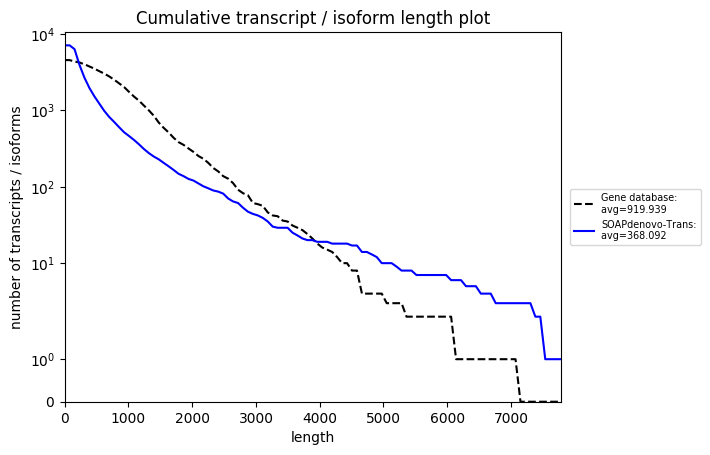
\includegraphics[width = \linewidth]{/mnt/dessertlocal/projects/transcriptome_assembly/review/evaluation/rna-quast/hsa/comparison_output/transcript_length.png}
\caption{Plot showing cumulative transcript length distribution. Each point represents the number of transcripts in the assembly with the corresponding length or longer; black dashed line corresponds to the database isoforms; the plot is given in logarithmic scale.}
\end{figure}
\FloatBarrier
\clearpage


\begin{figure}[t]
\centering
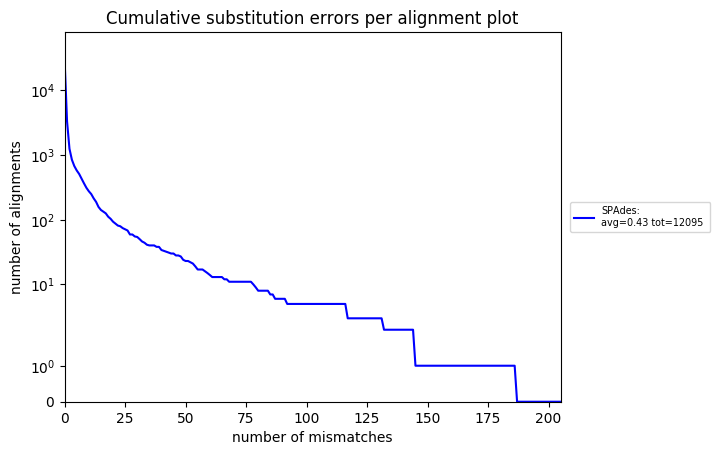
\includegraphics[width = \linewidth]{/mnt/dessertlocal/projects/transcriptome_assembly/review/evaluation/rna-quast/hsa/comparison_output/mismatch_rate.png}
\caption{Plot showing cumulative substitution errors per alignment distribution. Each point represents the number of alignments with the corresponding number of mismatches or greater; the plot is given in logarithmic scale.}
\end{figure}
\FloatBarrier
\clearpage


\begin{figure}[t]
\centering
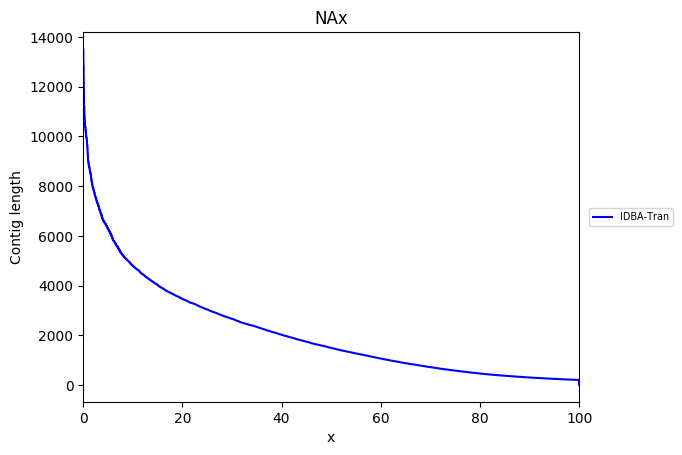
\includegraphics[width = \linewidth]{/mnt/dessertlocal/projects/transcriptome_assembly/review/evaluation/rna-quast/hsa/comparison_output/NAx.png}
\caption{Nx plot for transcripts. Nx is a maximal number $N$, such that the total length of all transcripts longer than $N$ bp is at least $x\%$ of the total length of all transcripts.}
\end{figure}
\FloatBarrier
\clearpage


\begin{figure}[t]
\centering
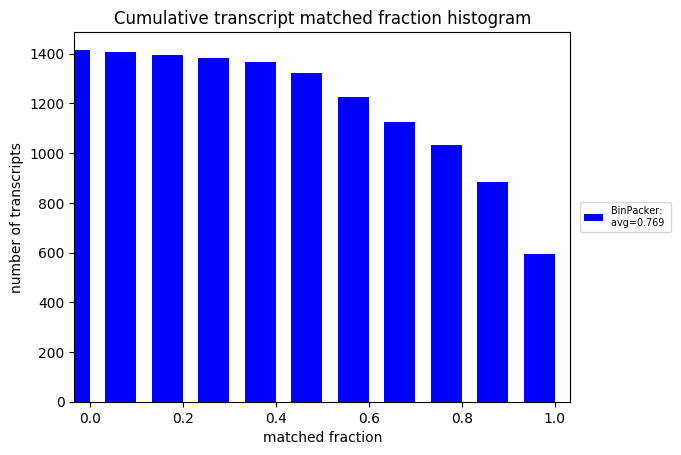
\includegraphics[width = \linewidth]{/mnt/dessertlocal/projects/transcriptome_assembly/review/evaluation/rna-quast/hsa/comparison_output/x-matched.png}
\caption{Plot showing cumulative transcript match histogram. Each bar represents the number of transcripts with matched fraction equal to or greater than the value on $x$ axis; transcript matched fraction is calculated as the number of its bases covering an isoform divided by the transcript length.}
\end{figure}
\FloatBarrier
\clearpage


\begin{figure}[t]
\centering
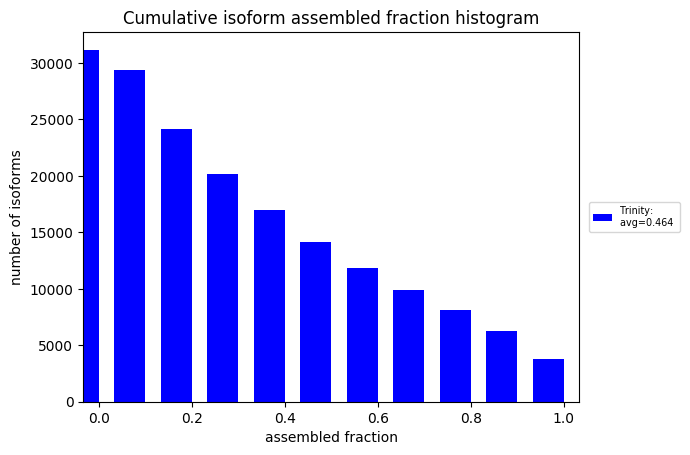
\includegraphics[width = \linewidth]{/mnt/dessertlocal/projects/transcriptome_assembly/review/evaluation/rna-quast/hsa/comparison_output/x-assembled.png}
\caption{Plot showing cumulative isoform assembly histogram. Each bar represents the number of isoforms with assembled fraction equal to or greater than the value on $x$ axis; isoform assembled fraction is calculated as the maximum number of captured by single assembled transcript bases divided by the total isoform length.}
\end{figure}
\FloatBarrier
\clearpage


\begin{figure}[t]
\centering
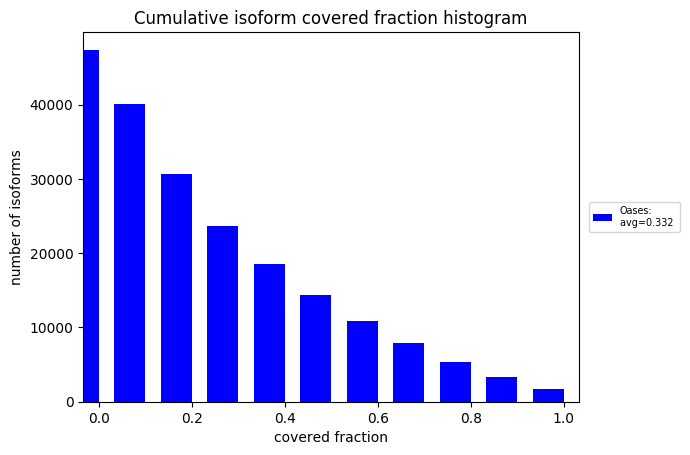
\includegraphics[width = \linewidth]{/mnt/dessertlocal/projects/transcriptome_assembly/review/evaluation/rna-quast/hsa/comparison_output/x-covered.png}
\caption{Plot showing cumulative isoform coverage histogram. Each bar represents the number of isoforms with covered fraction equal to or greater than the value on $x$ axis; isoform covered fraction is calculated as the number of covered bases (by all transcripts in the assembly) divided by the total isoform length.}
\end{figure}
\FloatBarrier
\clearpage


\end{document}
